\section{Program Logic for Location Virtualization}
\label{sec:logic}
% The predicate gen_heap_interp.
\newcommand{\gammaPred}{\delta}
\newcommand{\gammaPreds}{\delta\textsf{s}}
\newcommand{\rtv}{\textsf{rtv}}

\newcommand{\sumwalkabs}[3]{
  \ownGhost\gammaPred{\authfrag{\singletonMap{#1}{(#2, #3)}}}
}

\newcommand{\sumapaces}[2]{
  \ownGhost\gammaPreds{\authfrag{\singletonMap{#1}{#2}}}
}
\newcommand{\ptableabswalk}[1]{\mathcal{A}\textsf{bsPTableWalk}(#1)}
\newcommand{\ptablestore}{\theta}
Our reasoning principles are shaped around understanding the following perspectives on the vritual-memory abstraction:
\begin{enumerate}
\item \textit{logical representation of addressing}: we present physical memory addressing as separation-logic points-to relations.
\item \textit{sharing}: a bag of physical pages are reached through a set of physical page-table (L4-L1 page-tables) acceses that are shared amongst different virtual addresses. This sharing imposes constraints on giving a definition to the virtual-address in terms of physical (L4-L1) page-table memory accesses
\item \textit{context-agnostic-resources}: each virtual address is valid under a certain address-space, but it does not represent this \textit{knowledge} on its address-space. 
\item \textit{address-spaces as modal-contexts}: we call these context-agnostic resources (virtual-address pointstos) as \textit{context-resource}, and the context identfied by a unique \textit{namespace}, and  defining the truth for these context resources as \text{modal-context}
\item \textit{updating inter/intra address-spaces}: we present logical abstractions to enable allocating/updating pages in the existence of \textit{sharing}  
\item \textit{address-space switch as changing the "World" of truth}: switching from one address-space to another logically becomes introduction of \textit{context-resources} to the \textit{modal-context} under which they are valid, and loading \textit{context-resources} that are valid under the \textit{currently} loaded address-space
\end{enumerate}
Based on these perspectives, we coneptualize truth on an address-space through the contingency it exhibits: \textit{assertion P holds on this address-space indexed by its roots address}. Therefore, as a first step, we lift standard bi proposition to be indexed with $\mathcal{W}_{64}$ as shown in Figure \ref{fig:vprop}, and, most notably, all abstractions we explain in this section as part of our custom-tailored address-space logic are type $\textsf{vProp }\Sigma$.
\begin{figure}[!ht]
\[
\begin{array}{cl}
\textsf{vProp } \Sigma \; : \; \textsf{bi} \; \stackrel{{\triangle}}{:=} \mathcal{W}_{64} \rightarrow_{\textsf{b}} \textsf{iPropI } \Sigma
\end{array}
\]
\caption{$\textsf{vProp }\Sigma$: Root-Address Indexed Address-Space Proposition}
  \label{fig:vprop}
\end{figure}
%\subsection{Machine State under Address Translation}
%\label{sec:selectedinstrsemantics}
%Althought we give the complete set of operational semantics rule in \sref{appendix:movops}, It is worth building the intuition on the the way some of these rules bahave in the context of address translation. In fact $\readlval\maddr{\storememstar\crval}\locsf$ is unfoled into multiple physical memory lookups for the final page address retrieval -- i.e. address translation traversal as shown in Figure \ref{fig:pagetables}:
%\begin{itemize}
%\item top-level-address translation: with the given root address (64-bit $\crval$) of the address space, performs the address translation, handling the first level (to get the PML4 entry) itself. The next level table address is computed with the fetched PML4 offset value which exhibits itself as 9-bit offset in $\kw{maddr}$. \mytodo{iso: put move}
%\item translating from PML4 entry: performs the second level of address translation, to retrieve starting at the PML4 table entry, and interprets the PML4 entry that references a Page-Directory-Pointer Table (PDPT). We obtain the PDPT offset which exhibits itself as 9 bit offset in $\kw{maddr}$ to obtain the address of the next level page directory table (PDT) \mytodo{iso: put move}
%\item translating from PD entry: performs the third level of address translation, to retrieve starting at the PDP table entry, and interprets a PDPTE that references a PD table. Likewise, we obtain the PD offset which exhibits itself as 9 bit offset in $\kw{maddr}$ to obtain the address of the next level page directory table (PT) \mytodo{iso:put move }
%\item translate from PT entry: performs final level of address translation, starting from the PT entry, with a given 12 bit page offset, we can compute the physical address referencing $\locsf$ \mytodo{ismo: put mov}
%\end{itemize}
\subsection{Points-To Assertions}
\label{sec:pointsto}
We abstract physical memory addressing and registers naming with well-known separation logic assertion \textit{points-to} assertions.
\begin{enumerate}
\item Physical address points-to, $\pfpointsto\locsf\vpts\qfrac\ppts$
\item Register points-to, $\pfpointsto\rg\rv\qfrac\rpts$
\end{enumerate}
\paragraph{Register points-to} The assertion $\pfpointsto\rg\rv\rpts\qfrac$ ensures the ownership of the register $\rg$ naming the register value $\rv$. The fraction $\qfrac$ with value 1 asserts the unique ownership of the register mapping, and grants update permission on it, otherwise, any value $0 < \qfrac <1$ represents partial ownership granting readonly permission on the mapping.
\paragraph{Physical-Memory points-to} Our physical memory points-to relation in Figure \ref{fig:physicalpointsto} for a page table entry (e.g. \textsf{PDE} in Figure \ref{fig:pagetables}) abstracts masking -- $|^{52}$ for frame for and $|^{12}$ for offset -- through logical nested maps.  
\begin{figure}[!ht]
\[
\begin{array}{cl}
\pfpointsto\locsf\vpts\qfrac\ppts \stackrel{{\triangle}}{:=} & \nfpointsto{\mask\locsf\ft\generalentry}{\mask\locsf\tw\generalentry}\vpts\qfrac\naddr
\end{array}
\]
\caption{Physical Points-to with Nested Masking}
  \label{fig:physicalpointsto}
\end{figure}
Given the definition of physical page-pointsto assertion and the root address of virtual-address space kept in the control register \lstinline{cr3} as shown in Figure \ref{fig:pagetable},  one can build the physical address-translation for a virtual address (e.g. \textsf{va}) via abstracting the L4-L1 table traversal as the following:
\begin{itemize}
  \item Page Map Level-4 Translation (L4): Performs the first level address translation to get the PML4 entry (PML4E) in Figure \ref{fig:pagetables} by using the masks (\textsf{va}$|^{52}$(\lstinline{cr3}) to get the starting address of the PML4 table (PLM4T) and using the offset mask \textsf{va}$|^{12}$(\lstinline{cr3}). It is worth noting that our offset indices are 12 bits as all physical memory pointsto assertions has to satisfy being \textsf{\textit{aligned}}, e.g. [47-39] plus 3 alignment bits in Figure \ref{fig:pagetables}
    \[ \begin{array}{l}
      \hbox{(\TirNameStyle{{L4translate}})} \quad
      \exists \entryf \ldotp \nfpointsto{\mask\vaddr\ft\crthree}{\mask\vaddr\tw\crthree}\entryf\qfracfotsss\naddr
      \end{array}
      \]
  \item Page Directory Pointer Level Translation (L3): Performs the second level address translation to get the PDP entry (PDPE) in Figure \ref{fig:pagetables} by using the masks(\textsf{va}$|^{52}$(\textsf{PLM4E}) to get the starting address of the PDP table (PDPT) and using the offset mask \textsf{va}$|^{12}$(\textsf{PLM4E})
    \[\begin{array}{l}
    \hbox{(\TirNameStyle{{L3translate}})} \quad
    \exists \entrytr \ldotp \nfpointsto{\mask\vaddr\ft\entryf}{\mask\vaddr\tw\entryf}\entrytr\qfracfotss\naddr
    \end{array}
    \]
  \item Page Directory Table Level Translation (L2): Performs the second level address translation to get the PD entry (PDE) in Figure \ref{fig:pagetables} by using the masks(\textsf{va}$|^{52}$(\textsf{PDPE}) to get the starting address of the PD table and using the offset mask \textsf{va}$|^{12}$(\textsf{PDPE})
    \[ \begin{array}{l}
            \hbox{(\TirNameStyle{{L2translate}})} \quad 
       \exists \entrytw \ldotp \nfpointsto{\mask\vaddr\ft\entrytr}{\mask\vaddr\tw\entrytr}\entrytw\qfracfots\naddr
      \end{array}
      \]
  \item Page Table Level Translation (L1): Performs the second level address translation to get the PT entry (PTE) in Figure \ref{fig:pagetables} by using the masks(\textsf{va}$|^{52}$(\textsf{PDE}) to get the starting address of the Page table (PT) and using the offset mask \textsf{va}$|^{12}$(\textsf{PDE})
    \[ \begin{array}{l}
      \hbox{(\TirNameStyle{{L1translate}})} \quad
      \exists \entryo \ldotp \nfpointsto{\mask\vaddr\ft\entrytw}{\mask\vaddr\tw\entrytw}\entryo\qfracfot\naddr
      \end{array}
      \]
  \item Page Address Level Translation: Performs the second level address translation to get the physical page address in Figure \ref{fig:pagetables} by using the masks(\textsf{va}$|^{52}$(\textsf{PTE}) to get the starting address of the physical page address table and using the offset mask \textsf{va}$|^{12}$(\textsf{PTE})
    \[ \begin{array}{l}
      \hbox{(\TirNameStyle{{PageLebelAccess}})} \quad
      \exists \vpage \ldotp \nfpointsto{\mask\vaddr\ft\entryo}{\mask\vaddr\tw\entryo}\vpage\qfracone\naddr
      \end{array}
      \]
    
\end{itemize}
\begin{remark}[A Strong Definition for Virtual Memory Addressing]
  \label{rem:strongvmem}
  One could give a naive logical definition to the virtual mememory addressing as conjuctions of each level translation (Figure \fref{fig:strongvirtualpointsto}). The very first assurance our logical constructions need to be able assert is the \textit{existence} of the page table walk. Our naive attempt shown in Figure \ref{figure:strongvirtualpointsto}, we see that a virtual address with a certain fractional permissions at each level of the page-table walk gives us sound assurance of the path existence reaching to a page table entry, consequently, with a full-ownership of page address, we can obtain and update the value mapped value at this physical page address through our virtual memory address. 

\begin{figure*}
  \[
  \begin{array}{l}
\begin{array}{l}
  \vaddr\mapsto_{\textsf{t}}\{\textsf{q}\}\vpage\; : \mathsf{vProp} \; \Sigma \;  \stackrel{{\triangle}}{:=}  \lambda \crthree. \;\; \\
  \exists_{\entryf \;, \entrytr \;, \entrytw \;,\entryo} \ldotp 

  \ulcorner \textsf{aligned } \vaddr \urcorner \ast  \\
 \quad \textsf{L}_{4}\_\textsf{L}_{1}\_\textsf{PointsTo}(\crthree,\entryf,\entrytr,\entrytw,\entryo) \ast \nfpointsto{\mask\vaddr\ft\entryo}{\mask\vaddr\tw\entryo}\vpage\qfracone\naddr 
\end{array} \\
\\
\textsf{where   }\textsf{L}_{4}\_\textsf{L}_{1}\_\textsf{PointsTo}(\vaddr,\crthree,\entryf,\entrytr,\entrytw,\entryo) \stackrel{\triangle}{=} \\
 \qquad\qquad \nfpointsto{\mask\vaddr\ft\crthree}{\mask\vaddr\tw\crthree}\entryf\qfracfotsss\naddr \ast \\ 
 \qquad\qquad  \nfpointsto{\mask\vaddr\ft\entryf}{\mask\vaddr\tw\entryf}\entrytr\qfracfotss\naddr  \ast  \\
  \qquad\qquad \nfpointsto{\mask\vaddr\ft\entrytr}{\mask\vaddr\tw\entrytr}\entrytw\qfracfots\naddr \ast \\
  \qquad\qquad \nfpointsto{\mask\vaddr\ft\entrytw}{\mask\vaddr\tw\entrytw}\entryo\qfracfot\naddr 
   \end{array}
\]
\caption{A Strong Virtual Points-to Relation}
\todo[inline]{These fractions aren't quite right (though I see you added the variance between levels), I can walk you through in our meeting tomorrow.}
  \label{fig:strongvirtualpointsto}
\end{figure*}
\end{remark}
%then we reach to a physical page addr (e.g. \textsf{pa}) 
%\[  \paddr\mapsto_{\textsf{a}}\{1\}\vsome \ast \nfpointsto{\mask\vaddr\ft\entryo}{\mask\vaddr\tw\entryo}\vpage\qfrac\naddr \]

  \subsection{Aliasing/Sharing Physical Pages}
  \label{sec:sharingpages}  
  One might have already observed that the virtual points-to definition shown in Figure \ref{fig:strongvirtualpointsto} is too strong to specify virtual memory operations updating a page table entry. To speak more concretely, the fractional permissions on the page-table-walk assertion ($\textsf{L}_{4}\_\textsf{L}_{1}\_\textsf{PointsTo}$ in Figure \ref{fig:strongvirtualpointsto}) \textit{only} assure the existence of the certain number of mappings -- 512 at each level -- abstracting virtual address translations, and updating any of these mappings would make the other mappings, address translations sharing the page table mappings. Therefore, we need to consturct logical abstractions ensuring sound updates to the page-table entries in the existence of sharing.
\begin{figure*}
\[
\begin{array}{l}
    \vaddr\mapsto_{\textsf{v,rtv}}\{\textsf{q}\}\vpage \stackrel{\triangle}{:=} 
    \exists \entryo \ldotp
    \sumapaces\rtv\delta \ast 
  \sumwalkabs\vaddr\qfrac\paddr \ast 
   \nfpointsto{\mask\vaddr\ft\entryo}{\mask\vaddr\tw\entryo}\vpage\qfracone\naddr
\end{array}
\]
\caption{Virtual-Pointsto for Sharing Pages}
  \label{fig:virtualpointstosharing}
\end{figure*}  
  One possible approach is to abstract away the physical page-table-walk pointsto ($\textsf{L}_{4}\_\textsf{L}_{1}\_\textsf{PointsTo}$ in Figure \ref{fig:strongvirtualpointsto}) from the virtual pointsto relation. To do so, we introduce the protocol separating read-only (fragmental) and authorative (full ownership) accesses to the page tables, specifically $\textsf{L}_{4}\_\textsf{L}_{1}\_\textsf{PointsTo}$. We realize this protocol by embedding it into an already existing \textsf{Iris}'s ghost-map (or view\_maps) construction
  \[\mathcal{A}\textsf{bsPTableWalk} \stackrel{\triangle}{=} \textsc{Auth} (\; \mathcal{W}_{64} \;\rightarrow_{\textrm{fin}} \;  (\mathcal{W}_{64} \; \rightarrow_{\textrm{fin}}\;  (\textsc{Frac }, \mathord{+}) \times (\textsc{Agree } \Loc,\mathord{=}) ))\]
 where
  \begin{itemize}
  \item we decorate the fragmental ownership of the ghost-map ($ \sumwalkabs\vaddr\qfrac\paddr$) with the physical $\textsf{L}_{4}\_\textsf{L}_{1}\_\textsf{PointsTo}$ whose ownership just ensures that the virtual address ($\vaddr$) is mapped to a page (referenced by $\paddr$)
  \item we place the authorative ownership $\mathcal{A}\textsf{PTableWalk}$ of the ghost-map in an address-space invariant ($\mathcal{I}$\textsf{ASpace} in Figure \ref{fig:peraspaceinvariant}) whose ownership grants sound update on the page table entries
  \end{itemize}

  \begin{figure*}
\[
\begin{array}{l}
  \mathcal{I}\textsf{ASpace} \stackrel{\triangle}{:=} \lambda \; \crthree \ldotp
  \exists\;\gammaPred \;\ldotp\; \ownGhost\gammaPred{\authfull{\ptableabswalk\ptablestore}} \ast \\
  \bigast{(\vaddr, \entryo)\in \ptablestore}{\exists\;(\entryf\;,\entrytr\;,\entrytw)\ldotp \textsf{L}_{4}\_\textsf{L}_{1}\_\textsf{PointsTo}(\vaddr,\crthree,\entryf,\entrytr,\entrytw,\entryo)}
\end{array}
\]
\caption{Global Address-Space Invariant}
  \label{fig:peraspaceinvariant}
  \end{figure*}
  
\begin{remark}[Exchanging Page-Table-Walk-Summarization Mappings (Tokens) under Mutation of Page Tables ]
  $\mathcal{A}\textsf{PTableWalk}$'s fragmental-ownership represents an individual key-value pair (per-virtual-address) which can be handled as a \textit{look-up} resource for an individual virtual address.
  To build more intuition on the convenience of this protocol, we can think of the use-case \textit{unmapping-pages}. Normally, in the existence of shared page-tables, we need to first collect all the fragmental map pairs, e.g. $\sumwalkabs\vaddr\qfrac\paddr$, then, after making sure of non-existence of \textit{sharing}, we can \textit{unmap} the page. In this case, it would be ok to put $\textsf{L}_{4}\_\textsf{L}_{1}\_\textsf{PointsTo}$ and $ \sumwalkabs\vaddr\qfrac\paddr$ side-by-side inside the virtual-pointsto definition in Figure \ref{fig:virtualpointstosharing}. However, this pattern of verifying is not only inconvenient due to requirement of extra bookkeeping, but also violates our soundness argument based on considering  mutation on the shared page-tables -- due to coalescing of page tables etc. --. In other words, physical $\textsf{L}_{4}\_\textsf{L}_{1}\_\textsf{PointsTo}$ sitting aside to  $ \sumwalkabs\vaddr\qfrac\paddr$ would be made invalid by any concurrent update on the physical page-table. So there should only be one physical memory resource inside the virtual pointsto definition: from physical page address to the value stored ($   \nfpointsto{\mask\vaddr\ft\entryo}{\mask\vaddr\tw\entryo}\vpage\qfracone\naddr$).
\end{remark}

%\subsection{Address-Space Abstraction}
%\label{sec:aspacemodal}

Relations amongst these logical constructions, for the sake making it clearly understood, outlined pictorially  in Figure \ref{fig:logicaladdrspace}:
\begin{itemize}
\item a global address space invariant (solid round square labelled as $\mathcal{I}$\textsf{ASpace} in Figure \ref{fig:logicaladdrspace}) asserting the authorative ownership (i.e. update capability), $\ownGhost\gammaPred{\authfull{\ptableabswalk\ptablestore}}$, of the ghost map -- shown as solid-round-head arrow to $\mathcal{A}\textsf{PTableWalk}$ Figure \ref{fig:logicaladdrspace}
\item per-virtual-pointsto relation ((cutted round square labelled as \textsf{Virtual PointsTo} in Figure \ref{fig:peraspaceinvariant})) asserting the fragmental ownership of the ghost map, $\sumwalkabs\vaddr\qfrac\paddr$ \textit{represents} the fragmental-ownership (cutted-diamond-head arrow) of $\mathcal{A}\textsf{PTableWalk}$ 
\item there exists only one persistent authorative ownership ($\ownGhost\gammaPred{\authfull{\ptableabswalk\ptablestore}}$) for all fragmental ghost page-table-walk mapping ($\sumwalkabs\vaddr\qfrac\paddr$) shown as double-ended solid arrow 1 to N imposing the update protocol
\end{itemize}

\begin{figure}
   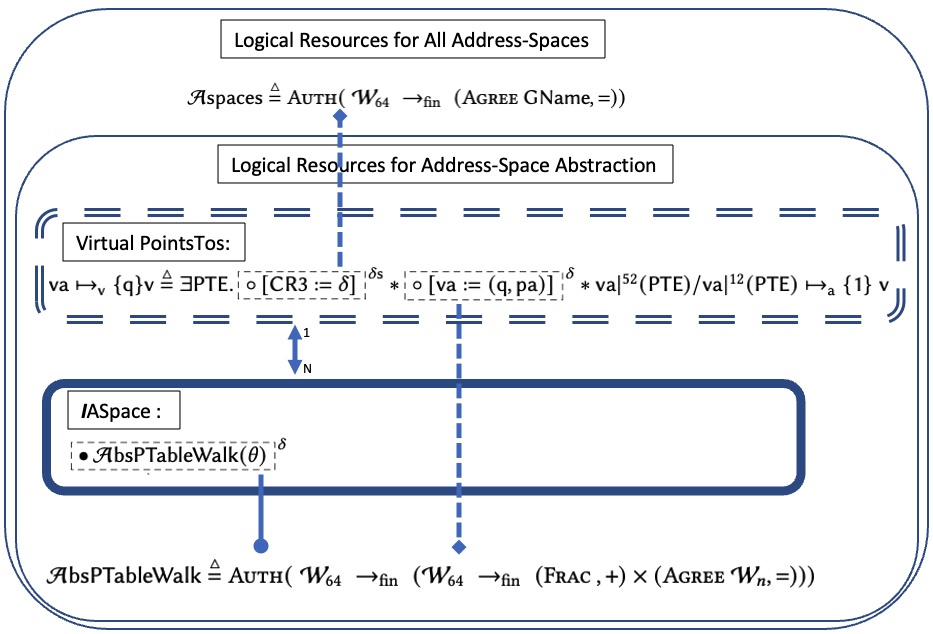
\includegraphics[width=0.75\columnwidth]{logical_addr_space.png}
  \caption{Logical Resources of Address-Space Abstraction}
  \label{fig:logicaladdrspace}
  \end{figure}

\subsection{Address-Space Management}
\label{sec:aspacemanagement}
So far, we have introduced logical abstractions for a single address space. However, \textsf{VMM} implementations handle more than one address-space which we abstract as a ghost map from root address of an address-space to a namespace labelling the address space
\[\mathcal{A}\textsf{spaces} \stackrel{\triangle}{=} \textsc{Auth} (\; \mathcal{W}_{64} \;\rightarrow_{\textrm{fin}} \; (\textsc{Agree } \mathsf{GName},\mathord{=}) ) \]

\paragraph{Valid Context-Resources} Fragmental ownership of $\mathcal{A}\textsf{spaces}$ ($\sumapaces\rtv\gammaPred$) conveys the fact that a current address-space ($\gammaPred$) is the one selected, i.e. loaded into the $\rtv$. This simple fact becomes essential when we observe it inside virtual-pointsto definition in Figure \ref{fig:virtualpointstosharing} and pictorially Figure \ref{logicaladdrspace}. Existence of this fragmental ownership ensures that the contextual resource, i.e. a virtual pointsto assertion, resides under the correct address-space, i.e. modal-context, that makes it valid.

\paragraph{Modal Resource Context\&Interaction with Ambient Logic \textsf{vProp}}
\label{sec:resourcecontext}
The relation between the address-space and and the validity of virtual-pointsto assertions exhibits itself as a contingency, i.e. \textit{"a certain virtual-pointsto facts whose validity is indexed by the root address of an address space"}. But, what sort of convenience this pattern provides when we do reasoning about more than one address-space.

In Figure \ref{fig:addrswitch}, we see two different address-spaces rooted at R0 and R1 in the pre/post condition. To be put into words, while switching an address-space by executing \lstinline|mov_ctl|) updating the  \lstinline|cr3|, it is expected to mention resources of two different address-spaces in the specification. In the precondition,  \lstinline|cr3| is loaded with R0 and all the virtual-pointsto assertions $a_0 \mapsto_{\textsf{v}}p_0$ and $a_1 \mapsto_{\textsf{v}}p_1$ are in the current-view of the memory and valid in the ambient logic \textsf{vProp}. The other address-space with the root address R1 has its own resources ($b_0 \mapsto_{\textsf{v}}p_3$ and $b_1 \mapsto_{\textsf{v}}p_4$) which are invalid under the current address space rooted at R0. This pattern of specification requires resources being mentioned under the \textit{world} they are valid, i.e. a modal-framing within the specification. Once the current address-space becomes the one with root address R1, i.e.  \lstinline|cr3| is loaded with R1, the context-resources $b_0 \mapsto_{\textsf{v}}p_3$ and $b_1 \mapsto_{\textsf{v}}p_4$ are loaded into the current-view of the memory, and all the other resources that are valid under R0 are introduced into the modal context rooted at R0
\begin{figure}

\[
  \begin{array}{l}
    \hbox{(\TirNameStyle{ModalAddressSpace)}} \qquad
         [r](P) \; \mathsf{vProp} \; \Sigma \; \stackrel{\triangle}{:=} \; \lambda \mathsf{P},\; \mathsf{P r}. 
  \end{array}
  \]
  \label{fig:modaldef}
  \end{figure}
  
\begin{figure}
\[
\begin{array}{l}
  \{ \textsf{cr3 } \mapsto_{r} R0 \ast a_0 \mapsto_{\textsf{v}}p_0  \ast a_1 \mapsto_{\textsf{v}}p_1  \ast [r1]\;( b_0 \mapsto_{\textsf{v}}p_3  \ast b_1 \mapsto_{\textsf{v}}p_4 )\}\\
  \qquad \qquad \qquad \qquad \qquad \mathsf{mov\_ctl} \;\; \texttt{cr3} \; \; R1\\

  \{ \textsf{cr3 } \mapsto_{r} R1 \ast [r0](a_0 \mapsto_{\textsf{v}}p_0  \ast a_1 \mapsto_{\textsf{v}}p_1)  \ast  b_0 \mapsto_{\textsf{v}}p_3  \ast b_1 \mapsto_{\textsf{v}}p_4 \}
  \end{array}
\]
  \label{fig:addrswitch}
  \end{figure}

\begin{remark}[The Choice of Modal Context, Contingency and  Pattern of Verification Context]
  \label{remark:pattern}
The truth on an address space, exhibits itself as a contingent truth: a location virtualization assertion (a virtual points-to in \ref{fig:virtualpointstosharing}),  happens to valid in the \textit{current world} (in the current address space), and switching address spaces pulls information out of one \textit{world} into the “current view” of memory, and leaves other assertions true relative to the previous address space.

Therefore, an address-space, as an abstraction, can be treated as naming the memory state as a modal frame and the choice of page table root as a world in Kripke-style semantics. Not suprisingly, transition between two address-spaces, then, can be just an entailment relation \textit{alternating} the \textit{named-state}

Being inspired by what hybrid logic \ref{} calls a satisfaction operator, which evaluates the truth of a predicate in a named alternative state (here, address space), we give a modal definition describing the truth of assertions for the resources (i.e. virtual pointsto relations) inside the address space. Ignoring the predicate types for a while, $[r]P$ in Figure \ref{fig:modaldef}, indicates that $P$ holds in the virtual address space rooted at $r$, the truth ($P$) on an address-space is indexed by the root page-table address $r$ of the address-space. In the rest of this section, we explain the structural aspects -- the modal resource context of address space modality -- , and how we lift the interaction of address-space modality with the ambient logic, i.e. separation logic as an entailment for specifying \textit{address-space-switch}.

Pragmatically, 
  \begin{enumerate}
  \item a modal context with its context-resources and picked contingency defines a modality (e.g. a address-space modality $[r]P$). For the convenience of verification, it enables focusing on the certain facts in the interest of reasoning (e.g. virtual pointsto relations in the current address-space)
  \item and, offloads the burden of individual bookkeeping of these facts (e.g. virtual pointsto relations per address-space) under different context (e.g. virtual pointsto relations in other address-spaces) via utilizing the \textit{summarization} aspect of the contingency it represents (e.g. other virtual pointsto relations are valid under other certain address-space page-table root addresseses).  
  \end{enumerate}
\end{remark}

\subsection{Considering Hoare Doubles in the Context of Switching Address-Space}
\subsubsection{Issues with Using Hoare Triples in Address-Space Specification}
\label{sec:issues}
An important subtlety arises with supporting \lstinline|mov|s into \lstinline|%cr3|. Consider the hypothetical rule:
\begin{mathpar}
\inferrule[Broken]{ }{
  \{P \ast \textsf{cr3}\mapsto_{r} \;r_1 \ast r \mapsto_{r} \;r_2 \ast [r_2](Q)\}
  \texttt{mov}~\texttt{\%cr3},~r%\lstinline|mov %cr3, r| 
  \{[r_1](P) \ast \textsf{cr3} \mapsto_{r} r_2 \ast r \mapsto_{r} r_2 \ast Q\}
}
\end{mathpar}
This rule captures the intuitive change of address space in a Hoare triple, rather than double, form. The problem with this is that it interacts quite poorly with the traditional frame rule and the modal flavor of virtual points-to assertions:
\begin{mathpar}
  \inferrule*[right=Frame]{
    \inferrule*[right=Broken]{ }{
    \{\mathsf{emp} \ast \textsf{cr3} \mapsto_{r} r_1 \ast r\mapsto_{r} r_2 \ast [r_2](Q)\}
    \texttt{mov}~\texttt{\%cr3},~r%\lstinline|mov %cr3, r| 
    \{[r_1](\mathsf{emp}) \ast \textsf{cr3} \mapsto_{r} r_1 \ast r \mapsto_{r} r_2 \ast Q\}
    }
  }{
    \{a\mapsto_\mathsf{v} x \ast \mathsf{emp} \ast \textsf{cr3}\mapsto_{r}r_1 \ast r \mapsto_{r}r_2 \ast [r_2](Q)\}
    \texttt{mov}~\texttt{\%cr3},~r%\lstinline|mov %cr3, r| 
    \{a\mapsto_\mathsf{v} x \ast [r_1](\mathsf{emp}) \ast \textsf{cr3} \mapsto_{r} r_1 \ast r \mapsto_{r} r_2 \ast Q\}
  }
\end{mathpar}
Notice that both the precondition and postcondition assert that $a\mapsto_\mathsf{v} x$ in the current address space, but we have no basis for concluding that address translation is preserved by the change of address space. So this derivation clearly leads to an unsound conclusion. This suggestss that the traditional frame rule and the Hoare triple presentation of the change-of-address-space rule cannot soundly coexist in the same system.
The heart of the problem is that while updating \lstinline|cr3| is \emph{physically} local, it globally changes the interpretation of virtual addresses. So it is simply unsound to frame around \lstinline|cr3| updates.

Switching to Hoare doubles resolves this problem because an under-appreciated subtlety of Hoare doubles is that typically \emph{there is no frame rule}. Instead each verification essentially includes a local frame that it passes to the next instructions (think continuation-passing style), giving each overall rule a \emph{global} (rather than local) precondition. For most rules this is not that important, but it does permit rules that have global effects on their preconditions.

This is then how we justify our actual rule for \lstinline|cr3| updates:
\begin{mathpar}
\inferrule[ChangeAddressSpace]{
  \{[r_1](P) \ast cr3 \mapsto_{r} r_2 \ast r \mapsto_{r} r_2 \ast Q\}\overline{is}
}{
  \{P \ast cr3 \mapsto_{r} r_1 \ast r \mapsto_{r} r_2 \ast [r_2](Q)\}
  \texttt{mov}~\texttt{\%cr3},~r;\;\overline{is}
  %\lstinline|mov %cr3, r| 
}
\end{mathpar}
Because the precondition on this rule is global, we avoid issues with framing.

If we wanted to consider a frame rule that would work for this logic, we could consider:
\begin{mathpar}
  \inferrule[Cr3Frame]{
    \{P\ast cr3=v\}\;C\;\{ Q \ast cr3=v\}
  }{
    \{R\ast P\ast cr3=v\}\;C\;\{ R \ast Q \ast cr3=v\}
  }
\end{mathpar}
By demanding that \lstinline|cr3| be held constant (or rather, at least restored to its original value) we could frame almost traditionally. In particular, this rule would work with framing around calls that might lead to address space switches, such as calling blocking operations in the kernel.

Readers familiar with dynamic frames~\cite{parkinson2011relationship} might find it useful to notice that a different perspective on this matter is that virtual points-to assertions are self-stable \emph{except} for changes in \lstinline|cr3|, so framing would then naturally require other means of holding \lstinline|cr3| constant (or saving and restoring it).
Virtual points-to assertions could be made self-stable by also giving them partial ownership over \lstinline|cr3| assertions, but this would require explicitly plumbing that ownership from \emph{all} assertions back to any place an address space change might occur; this would seem to be a far graver loss of modularity than this extra quirk in framing discussions.
\subsubsection{Defining Hoare Doubles for Address-Space Specification}
Based on the issues we discuss in Section \ref{sec:issues}, we make sure our Hoare-Double definition in Figure \ref{fig:wpddefinition} enables
\begin{itemize}
\item virtual-pointsto relations to be independent of \lstinline{cr3} ownership
\item and full-ownership of \lstinline to be propagated inside the \textsf{wpd\_def} in order to
\end{itemize}
This act of separation allows client-specification to be agnostic of \lstinline|cr3| physical resource, (i.e. \lstinline|cr3| $\mapsto_{\textsf{r}} \rtv$). The context-resource (virtual-pointsto) has only the \textit{knowledge} of being in a namespace in which it is valid ($\sumapaces\rtv\gammaPred$), nothing more.

In the rest of this, we explain how specifications of some selected \textsf{AMD64} instructions look like under the decisions made on the reasoning principles. All rules, e.g. the ones with different addressing mode, can be found in our artifact.

In the general outline of the proof in Figure \ref{wpdamd}, we see that each rule annotated with an address value ($\{\rtv\}$), i.e. a root address of an address-space, under which the resources mentioned in the specification are valid. Moreover, there is a frame resource $P$ in each rule.
\begin{figure} 
  \[
  \begin{array}{l}
    \textsf{wpd\_def e s E1 } \Phi \;\mathsf{ cr3val } : \textsf{iProp }\Sigma := \\
   \qquad ((\textsf{cr cr3}) \mapsto_{\textsf{r}} (\textsf{num cr3val)}) \textsf{ cr3val}) \ast (\Phi \textsf{ cr3val}) \wand \textsf{WP e E } @ \textsf{s ; E1 } \{\{\_, \textsf{True} \}\}
    \end{array}
  \]
\caption{Unfolded Hoare-Double Definition for \textsf{vProp} Logic }
\label{fig:wpddefinition}
\end{figure}

\begin{figure}
\begin{mathpar}
  \inferrule[WriteToRegFromReg | \{\textsf{rtv}\}]{
  \{P \ast r_d \mapsto_{r} \textsf{rvs} \ast r_s \mapsto_{r}\{q\} \textsf{ rvs} \}\;\overline{ is}
}{
  \{P \ast r_d \mapsto_{r} \textsf{rvd} \ast r_s \mapsto_{r}\{q\} \textsf{ rvs} \}
  \textsf{ mov}~\textsf{r}_d,~\textsf{r}_s;\;\overline{is}
  %\lstinline|mov %cr3, r| 
}
\\
\inferrule[WriteToPhysMemFromReg | \{\textsf{rtv}\}]{
  \{P \ast r_s \mapsto_{r}\{q\}  \textsf{rvs}  \ast r_a \mapsto_{r} \{q\} \textsf{ vaddr} \ast \textsf{vaddr} \mapsto_{\textsf{t}} \textsf{v} \}\;\overline{ is}  
}{
  \{P \ast r_s \mapsto_{r}\{q\}  \textsf{rvs}   \ast r_a \mapsto_{r}\{q\} \textsf{ vaddr} \ast \textsf{vaddr} \mapsto_{\textsf{t}} \textsf{rvs} \}
  \textsf{ mov}~\textsf{r}_a,~\textsf{r}_s;\;\overline{is}
}
\\
\inferrule[WriteToRegFromPhysMem | \{\textsf{rtv}\}]{
  \{P \ast r_d \mapsto_{r}  \textsf{v} \ast r_a \mapsto_{r} \{q\} \textsf{ vaddr} \ast \textsf{vaddr} \mapsto_{\textsf{t}} \textsf{v} \}\;\overline{is}
}{
  \{P \ast r_d \mapsto_{r}  \textsf{rvd} \ast r_a \mapsto_{r} \{q\} \textsf{ vaddr} \ast \textsf{vaddr} \mapsto_{\textsf{t}} \textsf{v} \}
  \textsf{mov}~\textsf{r}_d,~\textsf{r}_a;\;\overline{is}
}
\\
\inferrule[WriteToRegFromVirtMem | \{\textsf{rtv}\}]{
  \{P \ast \mathcal{I}\textsf{ASpace}\ast \mathcal{I}\textsf{ASpace} \ast r_d \mapsto_{r}  \textsf{v} \ast r_a \mapsto_{r} \{q\} \textsf{ vaddr} \ast \textsf{vaddr} \mapsto_{\textsf{v,rtv}} \textsf{v} \}\;\overline{is}
}{
  \{P \ast \mathcal{I}\textsf{ASpace}\ast r_d \mapsto_{r}  \textsf{rvd} \ast r_a \mapsto_{r} \{q\} \textsf{ vaddr} \ast \textsf{vaddr} \mapsto_{\textsf{v,rtv}} \textsf{v} \}
  \textsf{mov}~\textsf{r}_d,~\textsf{r}_a;\;\overline{is}
}
\\
\inferrule[WriteToVirtMemFromReg | \{\textsf{rtv}\}]{
  \{P \ast \mathcal{I}\textsf{ASpace}\ast r_s \mapsto_{r}\{q\}  \textsf{rvs}  \ast r_a \mapsto_{r} \{q\} \textsf{ vaddr} \ast \textsf{vaddr} \mapsto_{\textsf{v,rtv}} \textsf{v} \}\;\overline{ is}  
}{
  \{P \ast \mathcal{I}\textsf{ASpace}\ast r_s \mapsto_{r}\{q\}  \textsf{rvs}   \ast r_a \mapsto_{r}\{q\} \textsf{ vaddr} \ast \textsf{vaddr} \mapsto_{\textsf{v,rtv}} \textsf{rvs} \}
  \textsf{ mov}~\textsf{r}_a,~\textsf{r}_s;\;\overline{is}
}
\\
\inferrule[WriteToRegCtlFromReg | \{\textsf{rtv}\} / \{\textsf{rvs}\}]{
  \{P \ast r_s \mapsto_{r}\{q\}  \textsf{ rvs}  \}\overline{is}
}{
  \{P \ast r_s \mapsto_{r}\{q\}  \textsf{ rvs}   \}
  \textsf{mov}~\textsf{cr3},~r_s;\;\overline{is}
  %\lstinline|mov %cr3, r| 
}\\
\inferrule[WriteToRegFromRegCtl | \{\textsf{rtv}\}]{
  \{P \ast r_d \mapsto_{r} \textsf{rvs} \ast r_s \mapsto_{r}\{q\} \textsf{ rvs} \}\;\overline{ is}
}{
  \{P \ast r_d \mapsto_{r} \textsf{rvd} \ast r_s \mapsto_{r}\{q\} \textsf{ rvs} \}
  \textsf{ mov}~\textsf{r}_d,~\textsf{r}_s;\;\overline{is}
  %\lstinline|mov %cr3, r| 
}
\end{mathpar}
\caption{Reasoning Rules for Selected \textsf{AMD64} Instructions}
\label{fig:wpdamd}
\end{figure}
\subsubsection{Memory To Register}
In Figure \ref{fig:wpdamd}, we see the rules for updating the memory address ($r_a$). To do so, we essentially need page-table-walk pointsto ($\textsf{L}_{4}\_\textsf{L}_{1}\_\textsf{PointsTo}$ in Figure \ref{fig:strongvirtualpointsto}) to locate the value to be written. We mainly have two options to achieve this. 
\paragraph{Physical Memory To Register} First one is to use  page-table-walk pointsto ($\textsf{vaddr} \mapsto_{\textsf{t}} \textsf{v}$), which is consists of all-physical page-table memory assertions, to prove the page-table traversal \textsf{AMD64} implements, update the register $r_d$ the value obtained ($\textsf{v}$) as shown in Figure (\TirNameStyle{WriteToRegFromPhysMem}). By doing so, we expose the resources ($\textsf{L}_{4}\_\textsf{L}_{1}\_\textsf{PointsTo}$) needed only for the proof of \textsf{AMD64} page-table traversal to the client of the rule. This breaks the modularity of reasoning we want to maintain in location virtualization.
  \paragraph{Virtual Memory To Register}  Therefore, we would like to use a virtual-pointsto assertion ($\textsf{vaddr} \mapsto_{\textsf{v},\textsf{rtv}}$), which hides physical resources needed for the proof of page-table-traversal from the client, to obtain the the value ($\textsf{v}$) to update the register $r_d$ as shown in Rule (\TirNameStyle{WriteToRegFromVirtMem}). While doing the proof of page-table-traversal with a given virtual-pointsto definition in Figure \ref{fig:virtualpointstosharing}, we unfold and obtain our token ($\sumwalkabs\vaddr\qfrac\paddr$) to exchange for a physical-table mapsto assertion inside the $\mathcal{I}\textsf{ASpace}$ ($\textsf{L}_{4}\_\textsf{L}_{1}\_\textsf{PointsTo}$) in Figure \ref{fig:peraspaceinvariant}, and apply Rule (\TirNameStyle{WriteToRegFromPhysMem}).
\paragraph{Updating \lstinline|cr3|} Unlike other rules, \TirNameStyle{WriteToRegCtlFromReg} updates the root address of the address-space determining the validity of resources, $\{\rtv\} / \{\textsf{rvs}\}$.

